%! Author = antonio
%! Date = 9/6/24

\subsection{Evaluation}
\label{subsec:evaluation}

Starting with the model already tested, we go on to see how it behaves with another dataset which is the evaluation dataset.

\begin{figure}[h!]
    \centering
    \begin{subfigure}[b]{0.40\linewidth}
        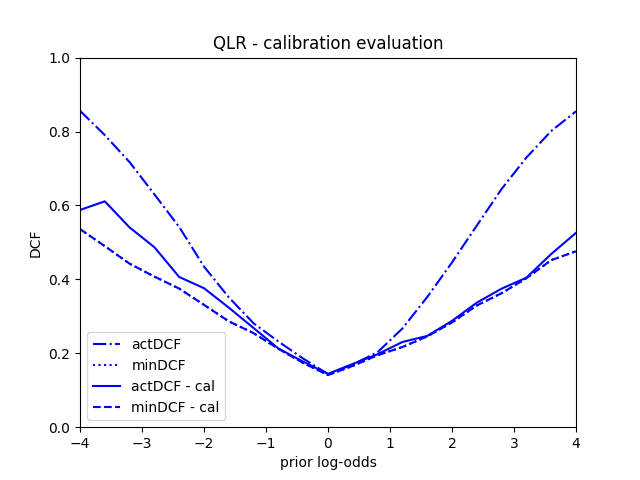
\includegraphics[width=\linewidth]{Lab/11. Lab 11/Images/Evaluation/01. QLR}
        \label{fig:QLREvaluation}
    \end{subfigure}
    \begin{subfigure}[b]{0.40\linewidth}
        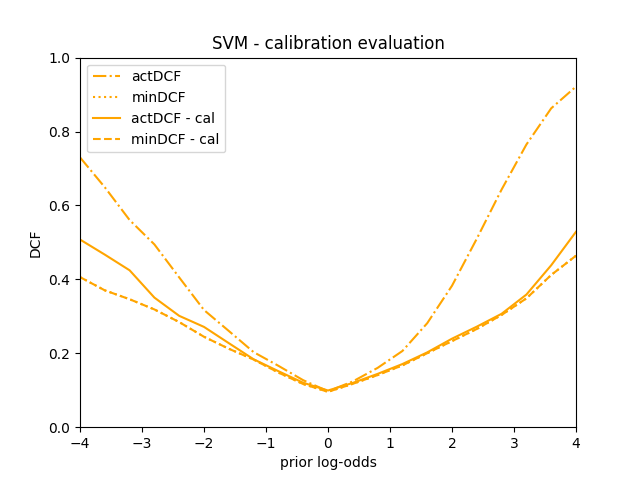
\includegraphics[width=\linewidth]{Lab/11. Lab 11/Images/Evaluation/02. SVM}
        \label{fig:SVMEvaluation}
    \end{subfigure}
    \begin{subfigure}[b]{0.40\linewidth}
        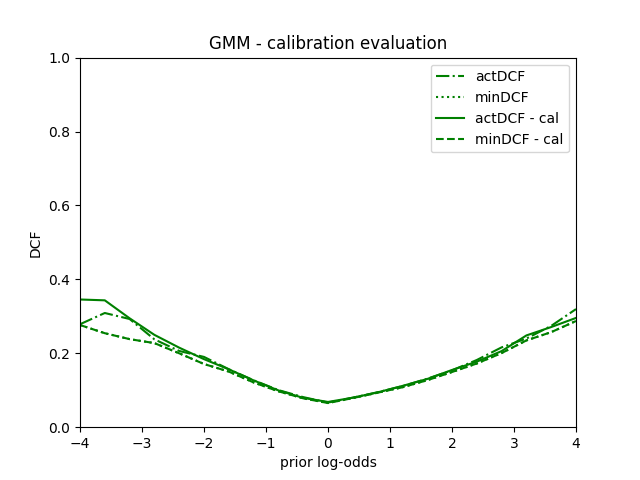
\includegraphics[width=\linewidth]{Lab/11. Lab 11/Images/Evaluation/03. GMM}
        \label{fig:GMMEvaluation}
    \end{subfigure}
    \begin{subfigure}[b]{0.40\linewidth}
        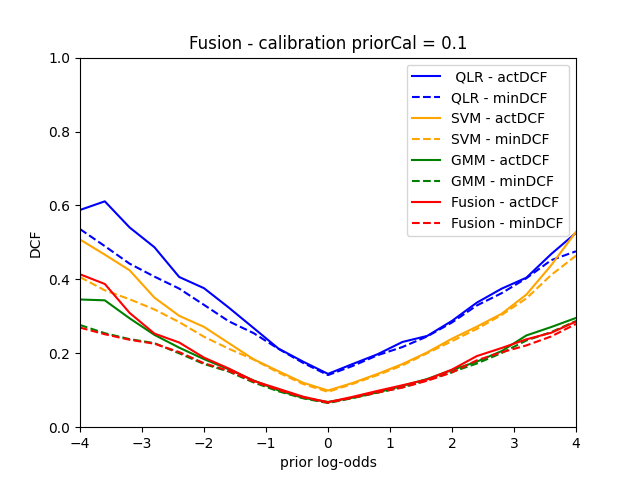
\includegraphics[width=\linewidth]{Lab/11. Lab 11/Images/Evaluation/04. Fusion}
        \label{fig:FusionEvaluation}
    \end{subfigure}
    \caption{Shows result of each model before and after calibration with the evaluation dataset}
    \label{fig:BestConfigurationCalibrationEvaluation}
\end{figure}

The \autoref{fig:BestConfigurationCalibrationEvaluation} shows the result of each model before and after calibration with the evaluation dataset
and a \(\tilde{\pi} = 0.1\).

\begin{table}[h!]
    \centering
    \begin{tabular}{>{\centering\arraybackslash}p{2.9cm} >{\centering\arraybackslash}p{2.9cm} >{\centering\arraybackslash}p{2.9cm} >{\centering\arraybackslash}p{2.9cm}}
        \toprule
        & \multicolumn{3}{c}{\textbf{Uncalibrated Models [minDCF - actDCF]}} \\
        \midrule
        \textbf{QLR} & \multicolumn{3}{c}{0.3515 - 0.4935} \\
        \textbf{SVM} & \multicolumn{3}{c}{0.2636 - 0.3634} \\
        \textbf{GMM} & \multicolumn{3}{c}{0.1838 - 0.1953} \\
        \midrule
        \midrule
        & \multicolumn{3}{c}{\textbf{Calibrated Models [minDCF - actDCF]}} \\
        \midrule
        & \(\tilde{\pi} = 0.1\) & \(\tilde{\pi} = 0.5\) & \(\tilde{\pi} = 0.9\) \\
        \midrule
        \textbf{QLR}    & 0.3515 - 0.3896       & 0.3515 - 0.3717       & 0.3515 - 0.3648       \\
        \textbf{SVM}    & 0.2636 - 0.2939       & 0.2636 - 0.2714       & 0.2636 - 0.2695       \\
        \textbf{GMM}    & 0.1838 - 0.2053       & 0.1838 - 0.2023       & 0.1838 - 0.2106       \\
        \midrule
        \textbf{Fusion} & 0.1865 - 0.2046       & 0.1831 - 0.2056       & 0.1828 - 0.2089       \\
        \bottomrule
    \end{tabular}
    \captionsetup{justification=justified,singlelinecheck=false,format=hang}
    \caption{Show minDCF and actDCF for different models before and after calibration on eval dataset}
    \label{tab:resultUnCalibratedAndCalibratedModelsOnEval}
\end{table}

The \autoref{tab:resultUnCalibratedAndCalibratedModelsOnEval} shows the minDCF and actDCF for different models before and
after calibration on the evaluation dataset.
From the values obtained, it is confirmed that GMM is again the method that gives the best performance, but Fusion also
gives good results that do not deviate much from those of GMM.\\
As seen above GMM is the best method for our case study, it might be interesting to see what happens by changing the convolution
type and the number of components on the evaluation dataset, leading to a better outcome.

\begin{table}[h!]
    \centering
    \begin{tabular}{>{\centering\arraybackslash}p{2.9cm} >{\centering\arraybackslash}p{2.9cm} >{\centering\arraybackslash}p{2.9cm}}
        \toprule
        \multicolumn{3}{c}{\textbf{GMM chosen (Diag, nc0 = 8, nc1 = 32)}} \\
        \midrule
        & \textbf{Uncalibrated} & \textbf{Calibrated} \\
        \midrule
        minDCF - actDCF & 0.1838 - 0.1953       & 0.1838 - 0.2053     \\
        \midrule
        \multicolumn{3}{c}{\textbf{GMM other (Diag, nc0 = 4, nc1 = 16)}} \\
        \midrule
        minDCF - actDCF & 0.1782 - 0.1900       & 0.1782 - 0.1970     \\
        \bottomrule
    \end{tabular}
    \captionsetup{justification=justified,singlelinecheck=false,format=hang}
    \caption{Show minDCF and actDCF for GMM chosen and another}
    \label{tab:GMMVSAnother}
\end{table}

